\begin{figure}
    \centering
    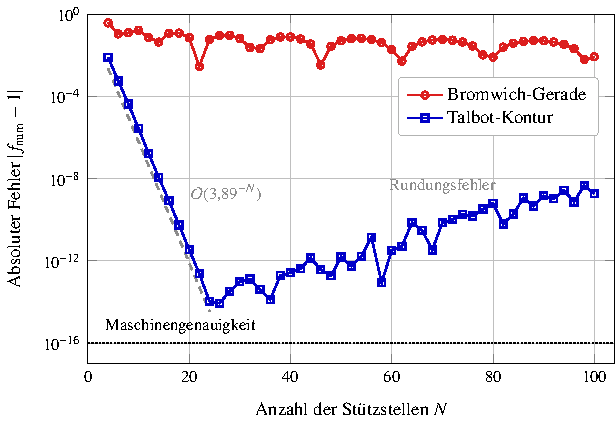
\includegraphics{papers/laplace/images/konvergenz_vergleich.pdf}
    \caption{Konvergenzvergleich der numerischen Inversion für
    $F(s) = \frac{1}{s}$ bei festem $t$:
    absoluter Fehler gegen die Anzahl der Stützstellen $N$ in
    halblogarithmischer Darstellung.
    Die Quadratur auf der Bromwich-Geraden (rot) verbessert sich nur
    langsam, während die Trapezregel auf der Talbot-Kontur (blau)
    geometrisch mit der Rate $O(3{,}89^{-N})$ konvergiert und um
    $N \approx 30$ nahe an die Maschinengenauigkeit herankommt.
    Für noch grössere $N$ steigt der Fehler wieder leicht an, weil der
    Faktor $e^{st}$ am Konturscheitel den Rundungsfehler wie
    $\varepsilon \, e^{0{,}17 N}$ verstärkt.}
    \label{laplace:fig:konvergenz_vergleich}
\end{figure}
